\section{Preliminary Experiments}
\label{sec:experiment}

%% by comparing applying a model checker to original C language programs
%% with to abstracted behavior.

We conducted preliminary experiments to check feasibility and to
investigate potential issues in the current framework.  For the
following C programs, we extract the behavioral types manually in the
form of another C programs.
\begin{itemize}

\item \texttt{poker.c}: a program which models a poker game.  It
  randomly deals two cards, compares these two and then decides which
  wins.  We rewrite this program as \texttt{poker\_rw.c} without
  changing its meaning.
\item \texttt{database.c}: from website
  (http://c.learncodethehardway.org/book/ex17.html) by Zed Shaw,
  modeling a database.  It opens a database and performs some
  operations on the database (retrieve, delete and update data, or
  create a new database) and closes the database.  We rewrite this
  program as \texttt{database\_rw.c} without changing its meaning.
\item \texttt{gen\_init\_cpio.c} is a file from Linux kernel (version 3.18.1)
  \texttt{/usr/gen\_init\_cpio.c}.  It produces a binary file which
  performs on a file containing newline separated entries that
  describe the files to be included in the initramfs archive.  Also, we
  rewrite this program to \texttt{gen\_init\_cpio\_rw.c}.
  \item \texttt{decompress\_unlzo.c} is a file from Linux kernel (version 3.18.1)
    \texttt{/lib/decompress\_unlzo.c}.  This is a LZO decompressor for
    the Linux kernel.  We rewrite it to the file \texttt{decompress\_unlzo\_rw.c}
\end{itemize}

We apply a model checker on these programs to check the property --
the number of memory usage does not exceed the number of available
memory cells.  In order to do it, in a program, we fixed a global
number $n$ which denotes the number of available memory for
allocation, it will decrease 1 when doing allocation and increase 1
when doing deallocation; we insert an assertion statement, $assert(n
>= 0)$, to check if doing one more allocation when the $n$ has
decreased to $0$.

Table~\ref{tb:mcc} and Table~\ref{tb:mca} give the result.  All of the
experiments are done on a machine with an Intel(R) Core(TM) i7-3770
CPU @ 3.40GHz, 8MB cache and 3.76GB memory, running on Debian (kernel
version 2.6.32-5-amd64) and CPAchecker (version 1.3.4).

\begin{table}
  \scriptsize
\begin{tabular}{|c|c|c|c|c|c|c|}
\hline
& \multicolumn{6}{|c|}{\texttt{original programs}}  \\
\hline
 & $\sharp$\texttt{loc} & $\sharp$\texttt{fun} & \texttt{cpu time (total,sec)} & \texttt{memory (MB)} & \texttt{fixed num}& \texttt{verified result} \\
\hline
\texttt{poker.c} & 86 & 4 & 2.700 & 2797 & 4  & \texttt{TRUE}  \\
\hline
\texttt{poker\_rw.c} & 89 & 4 & 2.740 & 2800 & 4  & \texttt{TRUE}  \\
\hline
\texttt{database.c} & 153 & 10 & 12.010 & 2907 & 2  & \texttt{TRUE}  \\
\hline
\texttt{database\_rw.c} & 151 & 10 & 7.080 & 2907 & 2  & \texttt{TRUE}  \\
\hline
\texttt{gen\_init\_cpio.c} & 346 & 19 & 9.580 & 2809 & 2  & \texttt{TRUE}  \\
\hline
\texttt{gen\_init\_cpio\_rw.c} & 343 &19  & 4.850  & 2744  & 2  & \texttt{TRUE}  \\
\hline
\texttt{decompress\_unlzo.c} & 162 & 2  & 3.000  & 2806  & 2  & \texttt{TRUE}  \\
\hline
\texttt{decompress\_unlzo\_rw.c} & 92 & 2  & 2.650  & 2800  & 2  & \texttt{TRUE}  \\

\hline
\end{tabular}
\caption{Model checking on original C language programs}
\label{tb:mcc}
\end{table}

\begin{table}
  \scriptsize
\begin{tabular}{|c|c|c|c|c|c|c|}
\hline
&\multicolumn{6}{|c|}{abstracted behavior} \\
\hline
 &$\sharp$\texttt{loc} & $\sharp$\texttt{fun} & \texttt{cpu time (total,sec)} & \texttt{memory (MB)} & \texttt{fixed num} & \texttt{verified result} \\
\hline
\texttt{poker.c} & 16 & 4 & 1.980 & 2803 & 4  & \texttt{FALSE}  \\
\hline
\texttt{poker\_rw.c} & 18 & 4 & 2.020 & 2798 & 4  & \texttt{TRUE}  \\
\hline
\texttt{database.c} &  16 & 4 & 2.060 & 2800 & 2 & \texttt{FALSE} \\
\hline
\texttt{database\_rw.c} &  18 & 4 & 1.990 & 2737 & 2 & \texttt{TRUE} \\
\hline
\texttt{gen\_init\_cpio.c} & 16 & 4 & 2.020 & 2802 & 2  & \texttt{FALSE}  \\
\hline
\texttt{gen\_init\_cpio\_rw.c} & 18 & 4 & 2.000  & 2742  & 2  & \texttt{TRUE}  \\
\hline
\texttt{decompress\_unlzo.c} & 16 & 4 & 1.970  & 2738  & 2  & \texttt{FALSE}  \\
\hline
\texttt{decompress\_unlzo\_rw.c} & 18 & 4  & 2.000  & 2796  & 2  & \texttt{TRUE}  \\

\hline
\end{tabular}
\caption{Model checking on an abstracted behavior}
\label{tb:mca}
\end{table}

The meaning of each column is as follows.  The column \texttt{original
  programs} and \texttt{abstracted behavior} mean applying the model
checker to a original C language program and to abstracted behavior
respectively.  These two columns consist of several columns:
$\sharp$\texttt{loc} means the number of program locations;
$\sharp$\texttt{fun} means the number of functions in a program;
\texttt{cpu time (total)} means the total execution time of CPU in
seconds; \texttt{memory(MB)} means the number of virtual memory cells
consumed by model checker in \texttt{MByte}; \texttt{fixed num} means
the number of available memory cells for allocation; the \texttt{TRUE}
in the \texttt{verified result} column means the number of the memory
cells which a program consumes does not exceed the \texttt{fixed num},
otherwise it is \texttt{FALSE} which denotes overflow.

The results present in the these two tables show that the
resources required for model checking become smaller if applying model
checkers to the abstracted behavior, since the abstracted behavior
only consists of allocation and deallocation.

One thing we should notice in these two tables is that for the same
programs, the \texttt{verified result} should be the same when model
checking on original programs and abstracted behavior; but it is not,
for example, \texttt{database.c} has the \texttt{TRUE} in the
Table~\ref{tb:mcc} but the \texttt{FALSE} in the
Table~\ref{tb:mca}. The reason is that our approach, abstracted
behavior, may not correctly deal with some conditional statements
about allocation and deallocation. For example, the behavior of
\texttt{database.c} is $\mu\alpha.\Malloc;\Malloc;(((\Free + 0);\Free)
+ 0);\alpha)$, due to the choice type, it may perform like
$\mu\alpha.\Malloc;\Malloc;0;0;\alpha$, which means consuming unbound
number of memory cells. The rewritten \texttt{database\_rw.c}, which
does not change the semantics of original program, has the behavior
$\mu\alpha.(\Malloc;(\Malloc + \Free) + 0);\Free;\alpha)$ which
returns \texttt{TRUE} when doing model checking on it.


%% \begin{table}
%% \tiny
%% \begin{tabular}{|c|c|c|c|c|c|c|c|c|c|c|}
%% \hline
%% & \multicolumn{5}{|c|}{original programs} & \multicolumn{5}{|c|}{abstracted behavior} \\
%% \hline
%%  & $\sharp$loc & $\sharp$fun & cpu time (total) & memory (MB) & fixed num & $\sharp$loc & $\sharp$fun & cpu time (total) & memory (MB) & fixed num \\
%% \hline
%% linklist.c & 154 & 13 & 9.770 & 2943 & 6(true) & 20 & 4 & 3.190 & 2918 & 6(false) \\
%% \hline
%% linklst2.c & 140 & 13 & 25.620 & 2955 & 21(true) & 20 & 4 & 10.72 & 2945 & 21(false) \\
%% \hline
%% linkstack.c  & 87 & 10 & 10.830 & 2941 & 11(true) & 20 & 4 & 4.990 & 2916 & 11(false) \\
%% \hline
%% linkqueue.c & 119 & 11 & 13.110 & 2939 & 4(true) & 25 & 4 & 2.660 & 2919 & 4(false) \\
%% \hline
%% binarysorttree.c & 80 & 5 & 30.210 & 2950 & 10(true) & 19 & 4 & 5.130 & 2935 & 10(false) \\
%% \hline
%% database.c & 179 & 12 & 4.930 & 2922 & 3(true) & 21 & 4 & 2.760 & 2920 & 2(false) \\
%% \hline
%% ihex2fw.c & 202 & 7 & 23.490 & 2882 & 5(false) & 15 & 4 & 2.160 & 2797 & 5(false) \\
%% \hline
%% gen\_init\_cpio.c & 346 & 19 & 9.580 & 2809 & 1(true) & 15 & 4 & 2.160 & 2799 & 1(false) \\
%% \hline
%% \end{tabular}
%% %%\caption{My first table}
%% \end{table}

%% \begin{figure}
%%  \centering
%%  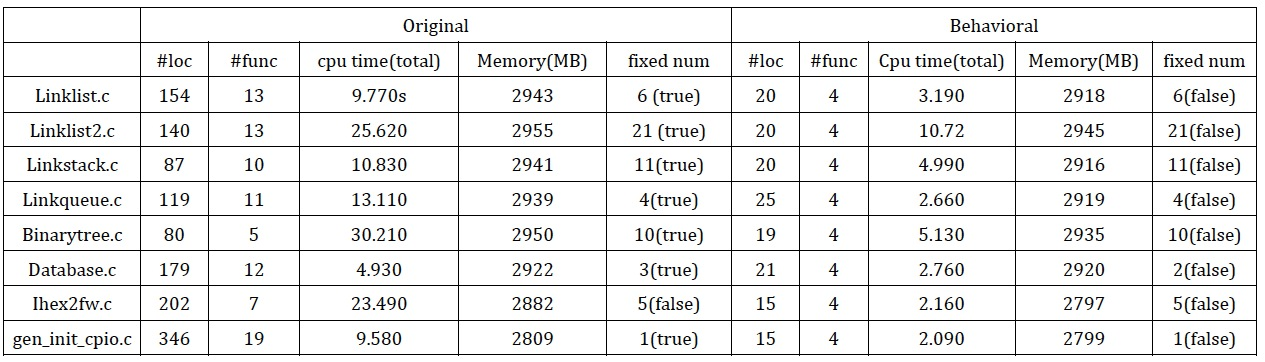
\includegraphics[width=14cm]{statistic.png}
%% \caption{Comparison}
%% \label{fig:statistic}
%% \end{figure}
